% file cmmr2023_template.tex 
% This is the LaTeX source for the instructions to authors using
% the LaTeX document class 'cmmr2023.cls' for contributions to
% the nternational Symposium on Computer Music Multidisciplinary Research 

\documentclass[runningheads,a4paper]{cmmr2023}
\usepackage{times}
\usepackage{amssymb}
\setcounter{tocdepth}{3}
\usepackage{graphicx}
\usepackage[hyphens]{url}
\newcommand{\keywords}[1]{\par\addvspace\baselineskip
\noindent\keywordname\enspace\ignorespaces#1}

\pagestyle{headings}

\begin{document}
\bibliographystyle{plain} % We choose the "plain" reference style
\bibliography{refs} % Entries are in the refs.bib file

\mainmatter  % start of an individual contribution

% first the title is needed
\title{The Unfinder: Finding and reminding in electronic music}

% a short form should be given in case it is too long for the running head
\titlerunning{The Unfinder}

% the name(s) of the author(s) follow(s) next
%
% NB: Chinese authors should write their first names(s) in front of
% their surnames. This ensures that the names appear correctly in
% the running heads and the author index.
%
\author{Rikard Lindell\inst{1}\and Henrik Frisk\inst{2} \thanks{KKS}}
%
% if the names of the authors are too long for the running head, please use the format: AuthorA et al.
\authorrunning{Lindell and Frisk}

% the affiliations are given next; don't give your e-mail address
% unless you accept that it will be published
\institute{Mälardalen University, School of Innovation, Design and Engineering and \\ Dalarna University, Dalarna Audiovisual Academy \and Royal College of Music, Institution of Composition, Conducting and Music Theory\\ \email{rikard.lindell@mdu.se}, \email{henrik.frisk@kmh.se}}
%
% NB: a more complex sample for affiliations and the mapping to the
% corresponding authors can be found in the file "llncs.dem"
% (search for the string "\mainmatter" where a contribution starts).
% "llncs.dem" accompanies the document class "llncs.cls".

\maketitle


\begin{abstract}
In this article we examine how we as composers of electronic music organize our material, files, samples, settings, and compositions, and how existing technologies fails to meet our expectations. This text is based on a pseudo-autobiographical pilot study, where we and one other composer wrote journal notes of a preparation for an improvisation based on previous works or other material. The notes were coded and analyzed using thematic analysis that resulted in six themes: \emph{Storage media}; \emph{Date, time, and remembering}; \emph{Matured material}; \emph{Structure, metadata, and collection of material}; \emph{Associations}; and \emph{Tool}. Despite the enormous amounts of storage capacity available, the practice we use today we bear similarities to Barreau and Nardi's \cite{Barreau1995} nearly 30-year-old article \emph{Finding and Reminding}. However, current operating systems were originally designed primarily to handle text files, the file system user interface has shortcomings in allowing for the kind of diversity and plethora of methods for storing and finding audio files in current music practices. Our study indicates that in order to support the way electronic music composers work, we need a usable, dynamic, plain, and transparent storage and material retrieval system.

\keywords{Personal Information Management, Information Retrieval, Artistic Sensibility, Electronic Music Composition, Thematic Analysis}
\end{abstract}

\section{Introduction}
Although we believe that it is feasible that the study of artistic practices may generate results that are of general value also outside of the field of the arts, any results that may be drawn from this particular study are only valid in relation to the artistic practices of the three participants. 
In their often cited and important paper in personal information management Barreau and Nardi \cite{Barreau1995} describe how users organize and retrieve files relying on the hierarchical file system. The similarities between the results of this almost 30 year old article, written at a time when storage devices were measured in mega-bytes at best, and the practice of digital artists in the present day with enormous amounts of digital material at their hands, still has relevance. In this paper we present the results of a pilot study of electronic musicians' personal information management of digital material: How do musicians organize their material (samplings, settings, naming files, etc.) on the various tools that they use before, during, and after a performance, and what are the needs that are not satisfied by existing technologies?

This question has a particular meaning in the genre of electronic music since there is often a lack of visual traces of what goes on in the sound producing engine. Whereas drummers, for example, moves their hands and hits cymbals that move. A laptop performer lacks a similar sense of immersion in performance: moving a finger, if even that, may result in a range of sonic effects, all of which lacks visual aspects.

Our study is part of a larger research project where we explore new designs to handle artistic material in electronic instruments, before, during, and after a performance. One of the central threads in the project is allowing for a widened view on information retrieval as a method. The hypothesis is that improved access to material creates an opportunity for a sense of immersion in electronic music. In order to address this we need to better understand what constitutes \emph{relevant} material in a musical performance in electronic music, and how this material is assembled.

This paper is based on a pre-study that we have performed partly to develop a reasonable method with which we can gather results about how a musician working with electronic instruments handle the material that is generated through their practice, both live and in the studio.
Both of the authors and one student at the Electroacoustic Music composition program at the Royal College of Music in Stockholm participated as subjects in the study. 

\section{Background}
The background to this study is the need to better understand how material that is generated in the process of composing music on a computer or with electronic instruments is handled by the user. How are files stored? How are they named? How are they retrieved? A  session can generate large amounts of material, this material, though often invisible to the listener, and even the musician, can contain structural information about the piece. Furthermore, it can be of interest to the musician to re-use the material in forthcoming projects. To approach this complex field we have chosen to study how we, in our musical practices, handle the situation and compare it to results in previous studies in personal information management.

As mentioned in the Introduction the paper Finding and Reminding: File Organization from the Desktop by Barreau and Nardi\cite{Barreau1995} is an important reference. It “suggests that the way information is used is a primary determinant of how it will be organized, stored, and retrieved.” They write that the users practice has a bigger impact on the strategies than the design of the system. Another finding they present is that the value and quality of the information decrease with time and that users give up on elaborate filing systems because in the end they do not yield enough value. 

Ravasio, Sch\"ar, and Krueger \cite{Ravasio2004} investigated how office personnel use their computers. In their study they found two overarching problems. First, the computer desktop interface itself and the users' dealings with the technology; and second, the way the hierarchical file system navigation tools failed to support the information management. Of specific interest to our study are their findings concerning users' problems that often the information was distributes into different parts of the system, such as files, e-mails, and bookmarks, when these disparate pieces of information formed parts of a larger whole. These complicated searching and backup procedures forced users to redundantly move material across different storage media. 

With the aforementioned paper being twenty years old, and the changes that cloud storage backup and ubiquitous WiFi and mobile internet connection has led to, one might conclude that this paper is no longer relevant. However, Wilken and Kennedy \cite{Wilken2021} recently found that people today still use and rely on portable storage devices, both for file sharing and for backup. File navigation activity still plays a crucial part in moving files across these different storage media.

Bergman et al. \cite{Bergman2012} suggests that sophistication of the organizational strategy makes a difference to the time it takes to retrieve files and that visual cues also speed up finding files. They also indicate that despite the advent of sophisticated tools for system wide text based search, such as Google Desktop, Catfish or Apple’s Spotlight, users still rely on file navigation for their information retrieval and personal information management. Another study by Horst and Sinanan \cite{horst2021} finds that some of the participants feel a strong sense of nostalgia, evoked from file navigation, towards old data which affects the way users deal with their material: the emotional relation to the material impacts on choices made concerning storage. This contradicts the suggestion by Barreau and Nardi \cite{Barreau1995} that old files loose value over time. 

Dupont et. al \cite{dupont2009} found that there was a lack of efficient systems for retrieving data: “the tools available today for browsing through large musical libraries hinders the creative process”, and “with the growing availability of multimedia content, there is a still larger demand for more flexible and efficient tools to access content and search for data”. This is consistent with several of the findings in the more general studies of personal information management and retrieval above. 

Recent contributions suggest that machine learning and results from the field of music information retrieval can support artists and supply artistic materials in performances \cite{ordiales2017,roma2021}. Here, Knees and Schedl \cite{knees16_contex_music_simil_index_retriev} showed that context-based music information retrieval methods in general outperform content-based methods, whereas, content-based methods capture qualities closer to the material.

%% Dinneen and Ilja Frissen (2020) personal traits. 

\subsection{Theory}
Contemporary music since the twentieth century, including popular music, is full of examples of how change is a quality in itself: unexpected turns, erratic behavior and unpredictability are virtues that have been revered and supported creating stylistic changes at an ever increasing rate, where in popular music there is an abundance of genres and sub-genres. This is most likely connected to the fact that artistic work in general is engaged in multiple methods and is governed by change and difference to a large degree.

Artistic practice in music, and in particular experimental electronic music, which is the style we are focusing on in this paper, encapsulates all the things musicians do when they are engaged in making music. There is no real distinction between composer and performer in this genre and the practice includes everything from thinking about making music and thinking back on past activities involving music to preparing for a performance or talking to a sound engineer. 
The artistic practice is guided by artistic sensibility which operates in a logic of non-conceptual free play where associations can shift rapidly. Ingman \cite{Ingman2022} defines artistic sensibility “as the sensitivity and capacity to appreciate and act upon concerns of or pertaining to art and its production”. Thompson \cite{Thompson2009} includes an intersubjective perspective into the definition of artistic sensibility and claims it “embodies the awareness of the self as an artist through the integration of artistic and aesthetic attributes toward self and other.” This awareness is of importance in this project as it extends not only to the other musicians that may be involved in the performance, but also to the material that the artist is handling. It contributes to “a certain freedom of responsiveness as the client's artistic sensibility pervades and informs affective and cognitive reactions to his or her internal process and the wider environment.” \cite{Thompson2009}. 
Even if the genre, context, economy, ethics, and social circumstances set the confines for what is possible, there may not be a set goal against which the results can be measured. The critical judgment needs to happen continuously. Even if activities are geared towards a general end objective, such as a concert, distinctive for artistic practices is that they may always change direction at any time.

Artistic practices may have much in common with, and be very similar to, other practices such as programming, engineering, publicizing and many other tasks, however artistic practices are distinct from these because they are governed by an artistic sensibility towards all materials in the project. 
Schön \cite{schon1983reflective} delineates this process as “a conversation with the material of a situation.” In our study we have considered the material to be the materials of a composition such as score, source code, sound patches, text, images, and recordings that can be stored in files. In conversation with the material, artistic practices pivot around methods of finding rather than creating, of uncovering rather than control, change rather than uniformity, and they are generally experiential rather than propositional.

\section{Method}
As part of a larger study where we engage with electroacoustic under graduate composition students, this pilot study includes one male student and the two authors as previously mentioned. 
One of the purposes here is to develop the method for a larger study in which gender balance, background, and genre are of importance. 
In the study all participants worked on a computer and a set of various software and hardware.
We kept a journal of the preparation for an improvisation based on material from previous works or other sources.
In a project journal the participants reflect on how they organizes their material, and in a final reflection to identify and describe advantages and disadvantages of the structure, or lack thereof, they  were using. Furthermore, we asked him to briefly describe an utopian optimal solution for how to organize material in a practice such as his own that would support the composition process. Because we as authors are also part of the electronic music community our perspective in this study is emic. According to Pike \cite{pike1967language}, this means analyzing the unique meanings and symbols used within a culture or group that we as researchers are part of. He argues that the understanding of a culture requires examining the language and communication methods from within. Our insight in the experiences and perspectives of the practices of electronic music composers allowed us to also understand the underlying assumptions and values. On the other hand there is a risk that we from our privileged perspective have assumptions that may mask events in the practice that we then fail to expose because they are, to us, self-evident. We managed this risk by staying open to the data we analyzed and by relying in the thematic analysis method \cite{maguire2017,braun2006}. In the written reflections in the study related to the information retrieval process and how material is organized the method is inspired by autoethnography \cite{ellis2004ethnographic}. Thus, the main data for this pilot study consists of the written reflections of three participants. Instead of proof by numbers we have cross-examined the qualitative data, and trusted in our reflections and in the thematic analysis method.

Thematic analysis \cite{maguire2017,braun2006} is a pragmatic method to guide and organize the interpretation of data performed in six steps: (1) become familiar with the data, (2) generate codes, (3) search for themes, (4) review themes, (5) define themes, and (6) write-up. We made the initial three steps individually, where we both analyzed the student’s journal and each other's journal. In the second step we relied on open coding without preset codes. To document initial ideas and interpretation of the codes and themes we wrote memos inspired by the Strauss and Glaser’s \cite{glaser2017} grounded theory method. We made the remaining three steps collaboratively. This allowed us to calibrate ourselves in the analysis of the student’s reflections and double check our codes and themes because we both looked at each other's texts where the interpretation, codes and themes, of an extract from the reflection could be discussed with its author. Initially we had seventeen, mostly semantic, themes \cite{maguire2017}, based on the explicit meaning of utterances. In the fourth and fifth step we used the initial memos, revised, and redefined the themes into latent themes \cite{maguire2017}) where the themes express underlying ideas and processes.

\section{Research ethics statement}
The study did not handle any sensitive personal data. To use the data produced in the study, we have obtained the explicit consent from the participant. The participant has certified voluntary participation, providing us the right to publish pseudonymized quotes from the journal and sample recordings that illustrate findings, and the participant has certified awareness of the study’s procedure. Quotations from the project journal have been presented pseudonymously. The data from the study is stored pseudonymously.

\section{Findings}
From the data and codes we initially found twelve themes where each theme was built from a few codes. These themes were further developed and focused into six themes: \emph{Storage media}; \emph{Date, time, and remembering}; \emph{Matured material}; \emph{Structure, metadata, and collection of material}; \emph{Associations}; and \emph{Tool}. Figure \ref{fig:findings_1} presents a model of these themes and their relative inter-connections, and the themes are described in the following. 

\subsection{Storage media}
\label{sec:storage}
This theme refers to the activity of dealing with storage media. Media types and media storage location are both aspects that are included, as explained by P2: “the resulting piece, when I believe it is worth it, is stored via SoundCloud or Vimeo”. The development of storage media impacts on the workflow of artists and P2 further comments upon the ways in which this development allowed for new practices. When audio files "were too large for the floppy discs” the relationships changed and “eventually I did not store anything except the recording to the fixed media” (P2). P3 comments that they “usually copy the whole directory [...] which is problematic and takes up disk space”. Economic awareness of disk space usage may impact on artistic processes. Storage media is at the very heart of the activities discussed here and is of central importance. It can stretch from discontinued media such as physical tapes and disks, hard drives and SSD disks, and online storage formats. P1 explains: “Hard drives, cassette tapes, USB sticks and memory cards are tucked away everywhere in the studio and the workflow takes shape there as well.” These types of storage media have a huge impact on the material and a sound file stored on one media may change to a significant degree if transferred to another, both in terms of its properties and the ways in which it can be interacted with. This theme is connected to the themes \emph{Structure, metadata, and collection of material}; \emph{Date, time and remembering}; and, \emph{Matured material}, see Figure \ref{fig:findings_1}, because all these themes are consequences of the design of, and interface for the hierarchical file system media storage.
%Today, the storage media size, measured in gigabytes or even terabytes, of the computer disks ought to be large enough for media sizes to be unimportant.

% However, the quotes in our study indicate otherwise and makes media the stage where electronic pieces are made.

\subsection{Date, time, and remembering}
\label{sec:date}
This theme relates to the navigation, structuring, sorting, and information management of content material based on time and date. For instance, P2 describes how files are organized in date order: “However, the bundle files are sorted in the date order. For more elaborate pieces that constitute a plethora of different files, sketches, samples files, images, source code for SuperCollider.” It also accounts for associations to when pieces were made, or locating files from date associations. \emph{Date, time and remembering} is important within the storage container for a work (see \emph{Structure and metadata, collection of material}) but also describes the organization of the works themselves. Furthermore, forgetting about content material is also a part of this theme explained by P1 as “what is lost or forgotten is not used”. P1 continues by describing how sorting based on date can help the rediscovery of such forgotten content: “Sometimes I use sorting principles for lists of folders like "last opened/modified" to see what's hiding among the storage devices.” Memory is obviously central to this kind of practice since all musical practices rely on memory and mnemonic associations, also on an overarching level. P3 describes how rememberance is a part of a performance: “The advantage with my method is that once I start to play, I know what kind of material I have to work with.” P2 comments that “I can more easily remember when I made a piece of music rather than what I called it” which hints at the organizational importance of date and time. Materials that have been forgotten or lost that are perceived in a new way related to, acousmatic listening \cite{Kane2014}, are directly connected to the theme of \emph{Matured material}. Figure \ref{fig:findings_1}, shows that this theme has a relationship to \emph{Matured material} where time alters the perception of the material. It is related to the theme \emph{Structure, metadata, and collection of material} where date and time is explicitly used to organise the material. This theme is also related to \emph{Associations} due to the date supported in current systems, and to media storage because of the current implementation support for creation, last edited, and last opened dates.

\subsection{Matured material}
\label{sec:matured}
This theme is about the phenomenon of materials and the way they change over time, such as files maturing as a function of change in the user's perception. This is illustrated by P1 in the following quote: “In my view, it is like having a wine cellar without an inventory list and that the work in the studio can be equated with collecting the bottles that can be thought of as working well together or in some other way picked out to be uncorked.” This may be both due to the altered perspective, and because the material has actually deteriorated expressed by P1 as in “files may be processed and/or they may retain their original appearance”. Furthermore, files can be reused and repurposed based on their matured artistic qualities. There is a natural connection between this theme and the \emph{Date, time and remembering} theme because the main operative structure here is the passing of time, see Figure \ref{fig:findings_1}. \emph{Matured material} is also related to Schaeffer's reduced listening \cite{Kane2014}, where time makes us forget the origin of, or the circumstances of the creation of the sound. This is poetically described by P1 as a Darwinian archive in which only the strong, or used, material survives. Matured material that resides in folders or on external drives, relates this theme to the \emph{Storage media} theme and to the \emph{Structure, metadata, and collection of material} theme, see also Figure \ref{fig:findings_1}.

\subsection{Structure, metadata, and collection of material}
\label{sec:structure}
This theme describes the organization of content and material in files. A common exemplification of this is where pieces and works are structured inside a container, or a folder in a file system. Within this container, however, the file order is often unstructured, and the structure of the files may instead rely on metadata, for instance, date, color tags, file type, location --- the cartesian position within a folder. This can be achieved loosely via the file manager tools of the operating system, as illustrated in the quote:  “Tags and color coding of files as well as combinations of these to be able to more easily navigate what is linked by association due to content or area of use. […] I use a hard drive where files are arranged in different formations purely graphically in a folder.” (P1). These associations between material files makes this theme related to the \emph{Associations} theme, files located on different hard drives relates to the media storage theme, and the use of date metadata relates this theme to \emph{Date, time, and remembering}, see Figure \ref{fig:findings_1}. Another, more rigid, method to organize content in the container formally is through a structured description, such as a makefile. As reflected on by P3, choosing a strict method like this impacts on the voice of software. (See more under the theme of \emph{Tool}). Maintaining structure may be difficult due to inconsistencies in file names and metadata. P3, however, comments that “the disadvantage is that it is difficult to use/reuse material in other projects” if all the project files are assembled in one container. To reuse parts of a project, or the parameter structure and relations within the project container, while preserving the integrity of the material; related to the theme \emph{Associations}, see Figure \ref{fig:findings_1}; it may be necessary to make copies of the entire container rather than copying individual files. This kind of organization is akin to the common paradigm of files in a DAW where, as commented by P2, “each song was a file or bundle that included everything for the piece”. P2 continues that “the disadvantage [with this method] is the lack of order inside each piece, in particular for the more elaborate and experimental works that include many different file formats.” Dynamic organization of content, where the work rather than the storage constitutes the semantic structure, with querying for metadata across all projects would support the reuse of content.

\subsection{Associations}
\label{sec:associations}
This theme is about various associations between media, files and other aspects of artistic production, or systems that may operate with such associations. In the following quote, the whole network of association within a piece, between it content, parameters, and external connections is reused:  “A composition is often based on presets from a previous project, but channels and connections go to new inputs. Control data with step patterns or start and stop points, pitch changes, or automated effect parameters and pans can be transferred from one thing to another, and in an improvisational/intuitive way create a whole reminiscent of the previous project because junctions between them are built into the technical infrastructure of the work.” (P1)
%In some cases this includes thoughts about how automated analyses based on feature extraction can contribute to creating associations. There is a need for dynamic query of content and association between parameters of compositions, and association between sound and image materials on the basis of parameters, and features, for instance frequency spectrum. A search engine could be designed that looks up sounds based on semantic descriptions. These kinds of content retrieval systems may contribute to surprising associations between material items that has not been seen or anticipated by the artist.
\begin{figure}
    \centering
    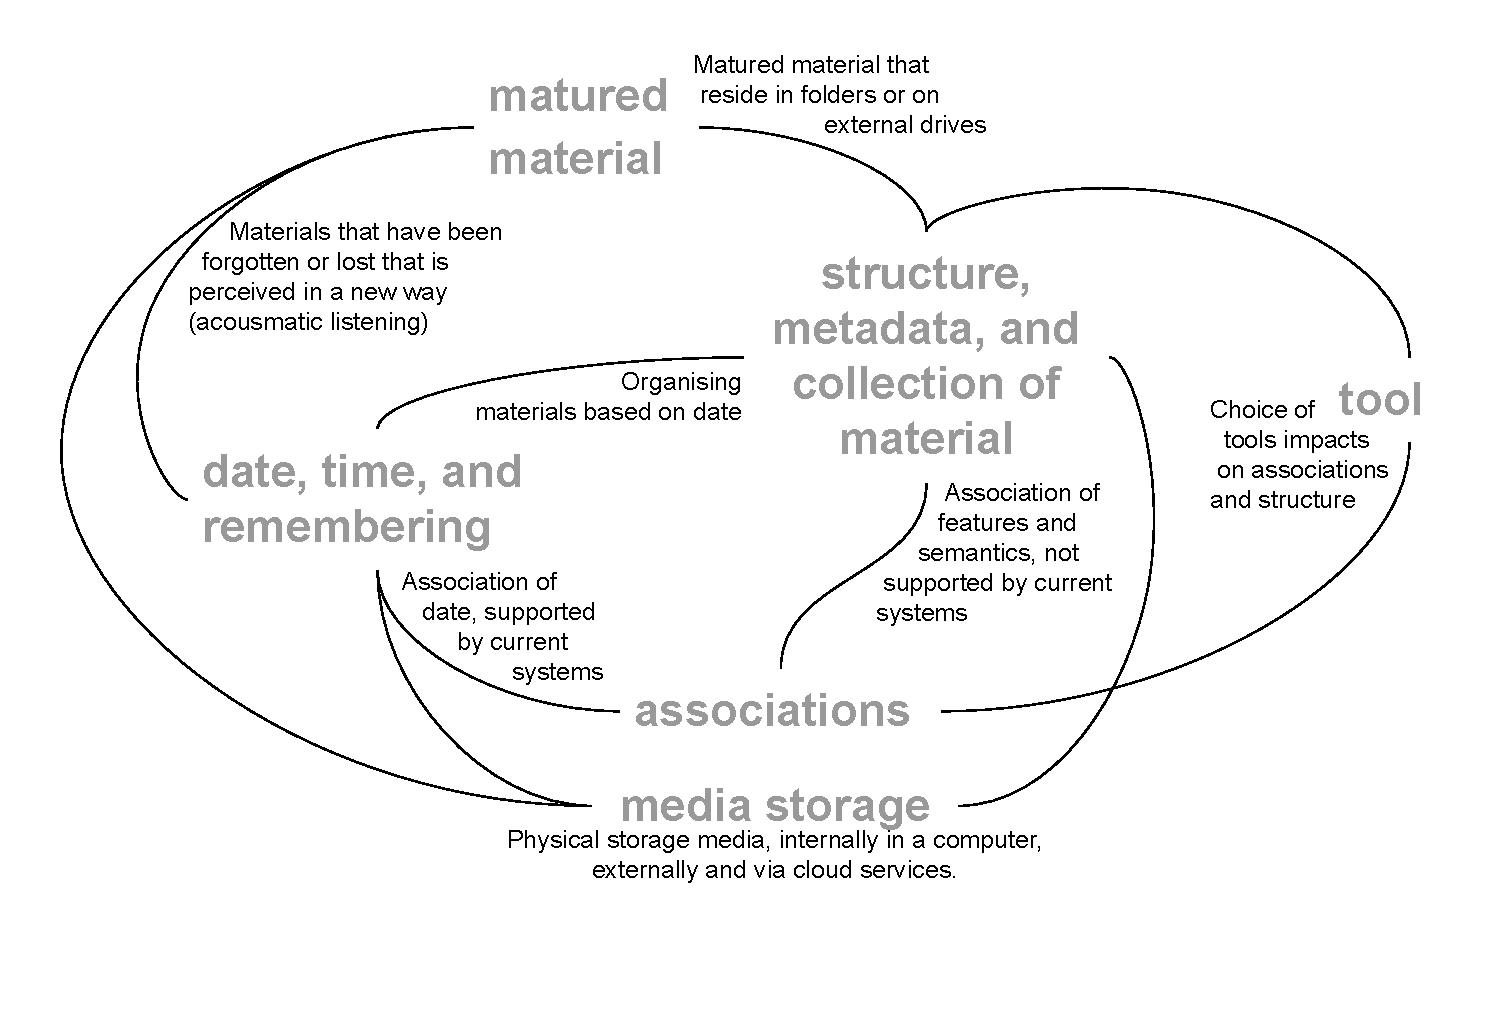
\includegraphics[width=\textwidth]{finding_reminding_no_stage_picture.pdf}
    \caption{This figure depicts the relationships between the themes. Each line represents an explicit relationship from the findings, where most of the relationships has a caption. For instance, the \emph{Date, time, and remembering} and \emph{Associations} themes have a relationship based on the file date metadata supported in current operating systems file navigation interfaces.}
    \label{fig:findings_1}
\end{figure}

In commonly used personal computer file navigation systems associations based on date are important, which is related to the \emph{Date, time, and remembering} theme, see Figure \ref{fig:findings_1}, whereas current information retrieval tools appear to not sufficiently support complex associations. P1 comments: “I sometimes use principles for sorting material that are related to ‘most recently opened/changed’ whereby I get information about what is hidden behind the structures of storage, and the result is often creative.” This may be understood as a method of choosing files that is not necessarily based on a musical association to the present material, but one that may generate surprising effects. The association in this case is temporal, and meta-structural (as in material often used are getting more exposure than others) rather than relational.

\subsection{Tool}
\label{sec:tool}
This theme concerns the tools, or lack thereof, in the artistic work for the management of content, which is either tool dependent, where the tool “dictates” how to handle content, or the lack of tool independent means for organizing and/or finding materials. Tools can also be aspects of a larger system for production such as a DAW that contains synths with presets, the use of which may also be considered a tool. Here the theme is related to \emph{Associations} theme, see Figure \ref{fig:findings_1},  because tools may impose or capture the associations of materials. A distinction between “tool” and “content” may be difficult to draw but is of interest in this context and is explored in the following quote: “It is a lengthy process if I want to change the sounds loaded, it's simply not possible to change loaded sounds in real time; they are hard coded.” (P3) Here, the tool makes it difficult to handle content. The actual practice of using an instrument may dictate the kinds of tools that are useful. In the case of a modular synthesizer, for example, a mobile phone camera may be useful to recreate a piece, whereas in programming a photo is less useful. A modular synthesizer, for example, depicts the possible means for documentation: “When I believe the patch of the modular synthesizer is worth saving, I use a notation or a patch description language that allows me to recreate a patch with some degree of precision.” (P2)
%Tool agnostic processes are those that do not depend on specific tools, such as the one imagined by a user asking for “a parameterized search engine for files that analyzes and categorizes the content of files in a particular directory and that furthermore suggests new systems for sorting different kinds of content.” (P1)
Recording and storing wave files in the file structure of the operating system is different from recording using a DAW that also provides the user with a management system, hence this theme is also related to the \emph{Structure, metadata, and collection of material} theme, see Figure \ref{fig:findings_1}.
%Information retrieval processes are either dependent on the tool, the DAW, for example, or the sound programming environment, or it may, as in the example above, be tool agnostic.

\section{Conclusions}
%- Our findings indicate that the electronic music composers that were part of this study are filing information according to systems of keywords, tags, and carefully architectured logical schemes. ... although there were systematic and logical schemes for the files in the systems, these were constructed based on the needs of the current project.

%Current file system of operating systems were originally constructed for primarily handling text files. Our study indicates that the file system user interfaces has deficiencies in allowing for a multiplicity of methods for storing and finding audio files. Because of these deficiencies, and to support how electronic composers work, we need to rethink the design of a usable, plain, and transparent storage system.

%Because of deficiencies in current operating systems' file system user interfaces, originally constructed for primarily handling text files, in allowing for a multiplicity of methods for storing and finding audio files there is a need to rethink the design of a usable, plain, and transparent storage system. 

%Music information is different from text or even images, where the first supports content-based information retrieval and indexed search, and the later has strong visual cues.




Wilken and Kennedy’s \cite{Wilken2021} notes on the nostalgia of data and its age may determine its value has links to the analysis under \emph{Matured material}, \emph{Storage media} (Section ~\ref{sec:storage}) and \emph{Date, time and remembering} (Section ~\ref{sec:date}) where in particular the discussion on “old wine” (see also Figure \ref{fig:findings_1}) suggests an objectification of the material. This aspect of nostalgia give rise to a further abstraction where the actual storage results in a representation of a memory and becomes more important than the data it holds: “archives are felt to be significant, even if the data is no longer accessible” \cite{Wilken2021} - the media is truly the message.

Our findings, in particular for the theme describing the \emph{Structure, metadata, and collection of material} (Section ~\ref{sec:structure}) indicate that electronic music composers are filing information according to systems of keywords, tags, and carefully architectured logical schemes.
This contradicts one of the key points of Barreau and Nardi \cite{Barreau1995}. Although our study shows that there are systematic and logical schemes for storing files by the users, these strategies were constructed based on the needs of the current project rather than on a general and reusable format. In other words, organization of files is structured according to the composition and production work, which is loosely in line with the conclusion by Wilken and Kennedy \cite{Wilken2021}. Barreau and Nardi are also stressing that “finding and reminding are intimately linked in users' practice and should be considered together” \cite{Barreau1995}. 
Storage arrangements today commonly range over a large number of different kinds of systems, such as cloud based, disks and USB-sticks, each with different levels of tangibility that offer different possibilities. These do indeed support individuality (see Section \ref{sec:storage}) but are commonly tied to the logic of the file system at hand. 
File access in current operating systems were originally constructed primarily for handling text files. 
According to aspects discussed in the themes \emph{Date and time, and remembering} (Section \ref{sec:date}), and \emph{Associations} (Section \ref{sec:associations}) relating to the organization of audio file and music information, our study indicates that the file system user interfaces has deficiencies in allowing for the kind of multiplicity of methods for storing and finding audio files that the participants in this study deploy. 
However, this study is mainly valid in relation to the three participants. Hence, our findings indicate the need for a larger study, with possibly more general results. Such a study could furthermore provide insight into other fields of creative practices but most importantly: We believe that there need to rethink the design of a usable, dynamic, plain, and transparent storage and material retrieval system to support how electronic music composers and performers work.

\begin{thebibliography}{4}
\bibitem{Barreau1995}Barreau, D. \& Nardi, B. Finding and reminding: file organization from the desktop. {\em ACM SigChi Bulletin}. (27):39--43 (1995)
\bibitem{Schnell2002}Schnell, N. \& Battier, M. Introducing composed instruments, technical and musicological implications. {\em Proceedings Of The 2002 Conference On New Interfaces For Musical Expression}. 156--160 (2002)
\bibitem{Ravasio2004}Ravasio, P., Schär, S. \& Krueger, H. In Pursuit of Desktop Evolution. {\em ACM Transactions On Computer-Human Interaction}. (11):156--180 (2004), http://dx.doi.org/10.1145/1005361.1005363
\bibitem{Wilken2021}Wilken, R. \& Kennedy, J. Everyday Data Cultures and Usb Portable Flash Drives. {\em International Journal Of Cultural Studies}. (25):192--209 (2021), http://dx.doi.org/10.1177/13678779211047917
\bibitem{Bergman2012}Bergman, O., Whittaker, S., Sanderson, M., Nachmias, R. \& Ramamoorthy, A. How do we find personal files?. {\em Proceedings Of The SIGCHI Conference On Human Factors In Computing Systems}. 2977--2980 (2012,5)
\bibitem{horst2021}Horst, H. \& Sinanan, J. Digital Housekeeping: Living With Data. {\em New Media \& Society}. (23):834--852 (2021), http://dx.doi.org/10.1177/1461444820953535
\bibitem{dupont2009}Dupont, S., Dubuisson, T., Urbain, J., Sebbe, R., D'Alessandro, N. \& Frisson, C. AudioCycle: Browsing Musical Loop Libraries. {\em 2009 Seventh International Workshop On Content-Based Multimedia Indexing, Content-Based Multimedia Indexing, 2009. CBMI '09. Seventh International Workshop On}. 73--80 (2009)
\bibitem{ordiales2017}Ordiales, H. \& Bruno, M. Sound recycling from public databases Another BigData approach to sound collections. {\em ACM International Conference Proceeding Series}. (2017)
\bibitem{roma2021}Xamb\'{o}, A., Roma, G., Roig, S. \& Solaz, E. Live Coding with the Cloud and a Virtual Agent. {\em NIME 2021}. (2021)
%\bibitem{roma2021}Xambo, A., Roma, G., Roig, S. \& Solaz, E. Live Coding with the Cloud and a Virtual Agent. {\em NIME 2021}. (2021)
\bibitem{knees16_contex_music_simil_index_retriev}Knees, P. \& Schedl, M. Contextual Music Similarity, Indexing, and Retrieval. {\em Music Similarity And Retrieval}. 133--158 (2016)
\bibitem{Ingman2022}Ingman, B. Artistic Sensibility is Inherent to Research. {\em International Journal Of Qualitative Methods}. (21) (2022,1)
\bibitem{Thompson2009}Thompson, G. Artistic sensibility in the studio and gallery model: Revisiting process and product. {\em Art Therapy}. (26)159--166 (2009)
\bibitem{schon1983reflective}Schon, D. {\em The Reflective Practitioner: How Professionals Think In Action}. 78--79 (Basic Books, 1983)
\bibitem{pike1967language}Pike, K. L. {\em Language in Relation to a Unified Theory of the Structure of Human Behavior}. (De Gruyter Mouton, 1967)
\bibitem{ellis2004ethnographic}Ellis, C. The ethnographic I: A methodological novel about autoethnography. (Rowman Altamira,2004)
\bibitem{maguire2017}Maguire, M. \& Delahunt, B. Doing a thematic analysis: A practical, step-by-step guide for learning and teaching scholars. {\em All Ireland Journal Of Higher Education}. (9) (2017)
\bibitem{Kane2014}Kane, B. Pierre Schaeffer, the Sound Object, and the Acousmatic Reduction. {\em Sound Unseen: Acousmatic Sound in Theory and Practice}. (Oxford University Press, 2014).
\bibitem{braun2006}Braun, V. \& Clarke, V. Using thematic analysis in psychology. {\em Qualitative Research In Psychology}. (3):77--101 (2006)
\bibitem{glaser2017}Glaser, B. \& Strauss, A. Discovery of grounded theory: Strategies for qualitative research. (Routledge, 2017)
%\bibitem{Khoo2007}Christopher S.G., K., Brendan, L., Caroline, E., Jamila, O., Hui-Hui, L. \& Sally, Y. How users organize electronic files on their workstations in the office environment: a preliminary study of personal information organization behaviour.. {\em Information Research: An International Electronic Journal}. \textbf{12}, 293 (2007)
%\bibitem{dinneen20_mac_users_do_it_differ}Dinneen, J. \& Frissen, I. Mac Users Do It Differently: the Role of Operating System and Individual Differences in File Management. {\em Extended Abstracts Of The 2020 CHI Conference On Human Factors In Computing Systems}. pp. nil (2020,4)

\end{thebibliography}



\end{document}
